\section{Design of PConv and FasterNet}
\label{sec:approach}
In this section, we first revisit DWConv and analyze the issue with its frequent memory access. We then introduce PConv as a competitive alternative operator to resolve the issue. After that, we introduce FasterNet and explain its details, including design considerations. 

\subsection{Preliminary}
DWConv is a popular variant of Conv and has been widely adopted as a key building block for many neural networks. For an input 
$ \mathbf{I} \in \mathbb{R}^{ c \times h \times w}$, DWConv applies 
$c$
filters
$ \mathbf{W} \in \mathbb{R}^{ k \times k} $
to compute the output 
$ \mathbf{O} \in \mathbb{R}^{ c \times h \times w}$.
As shown in~\cref{fig: PConv}(b), each filter slides spatially on one input channel and contributes to one output channel.
This depthwise computation makes DWConv have as low FLOPs as $ h \times w \times k^2 \times c$ compared to a regular Conv with
$ h \times w \times k^2 \times c^2$. While effective in reducing FLOPs, a DWConv, which is typically followed by a pointwise convolution, or PWConv, cannot be simply used to replace a regular Conv as it would incur a severe accuracy drop.
Thus, in practice the channel number
$c$ (or the network width) of DWConv is increased to 
$c'\left(c' > c\right)$
to compensate the accuracy drop, \eg, the width is expanded by six
times for the DWConv in the inverted residual blocks~\cite{sandler2018mobilenetv2}. This, however, results in much higher memory access that can cause non-negligible delay and slow down the overall computation, especially for I/O-bound devices. In particular, the number of memory access now escalates to 
\begin{equation}
  h \times w \times 2c' + k^2 \times c'\approx h \times w \times 2c',
  \label{eq:memory_access_DWConv}
\end{equation}
which is higher than that of a regular Conv, \ie,
\begin{equation}
  h \times w \times 2c + k^2 \times c^2 \approx h \times w \times 2c.
  \label{eq:memory_access_Conv}
\end{equation}
Note that the $h \times w \times 2c'$ memory access is spent on the I/O operation, which is deemed to be already the minimum cost and hard to optimize further.

\begin{figure}
    \centering
    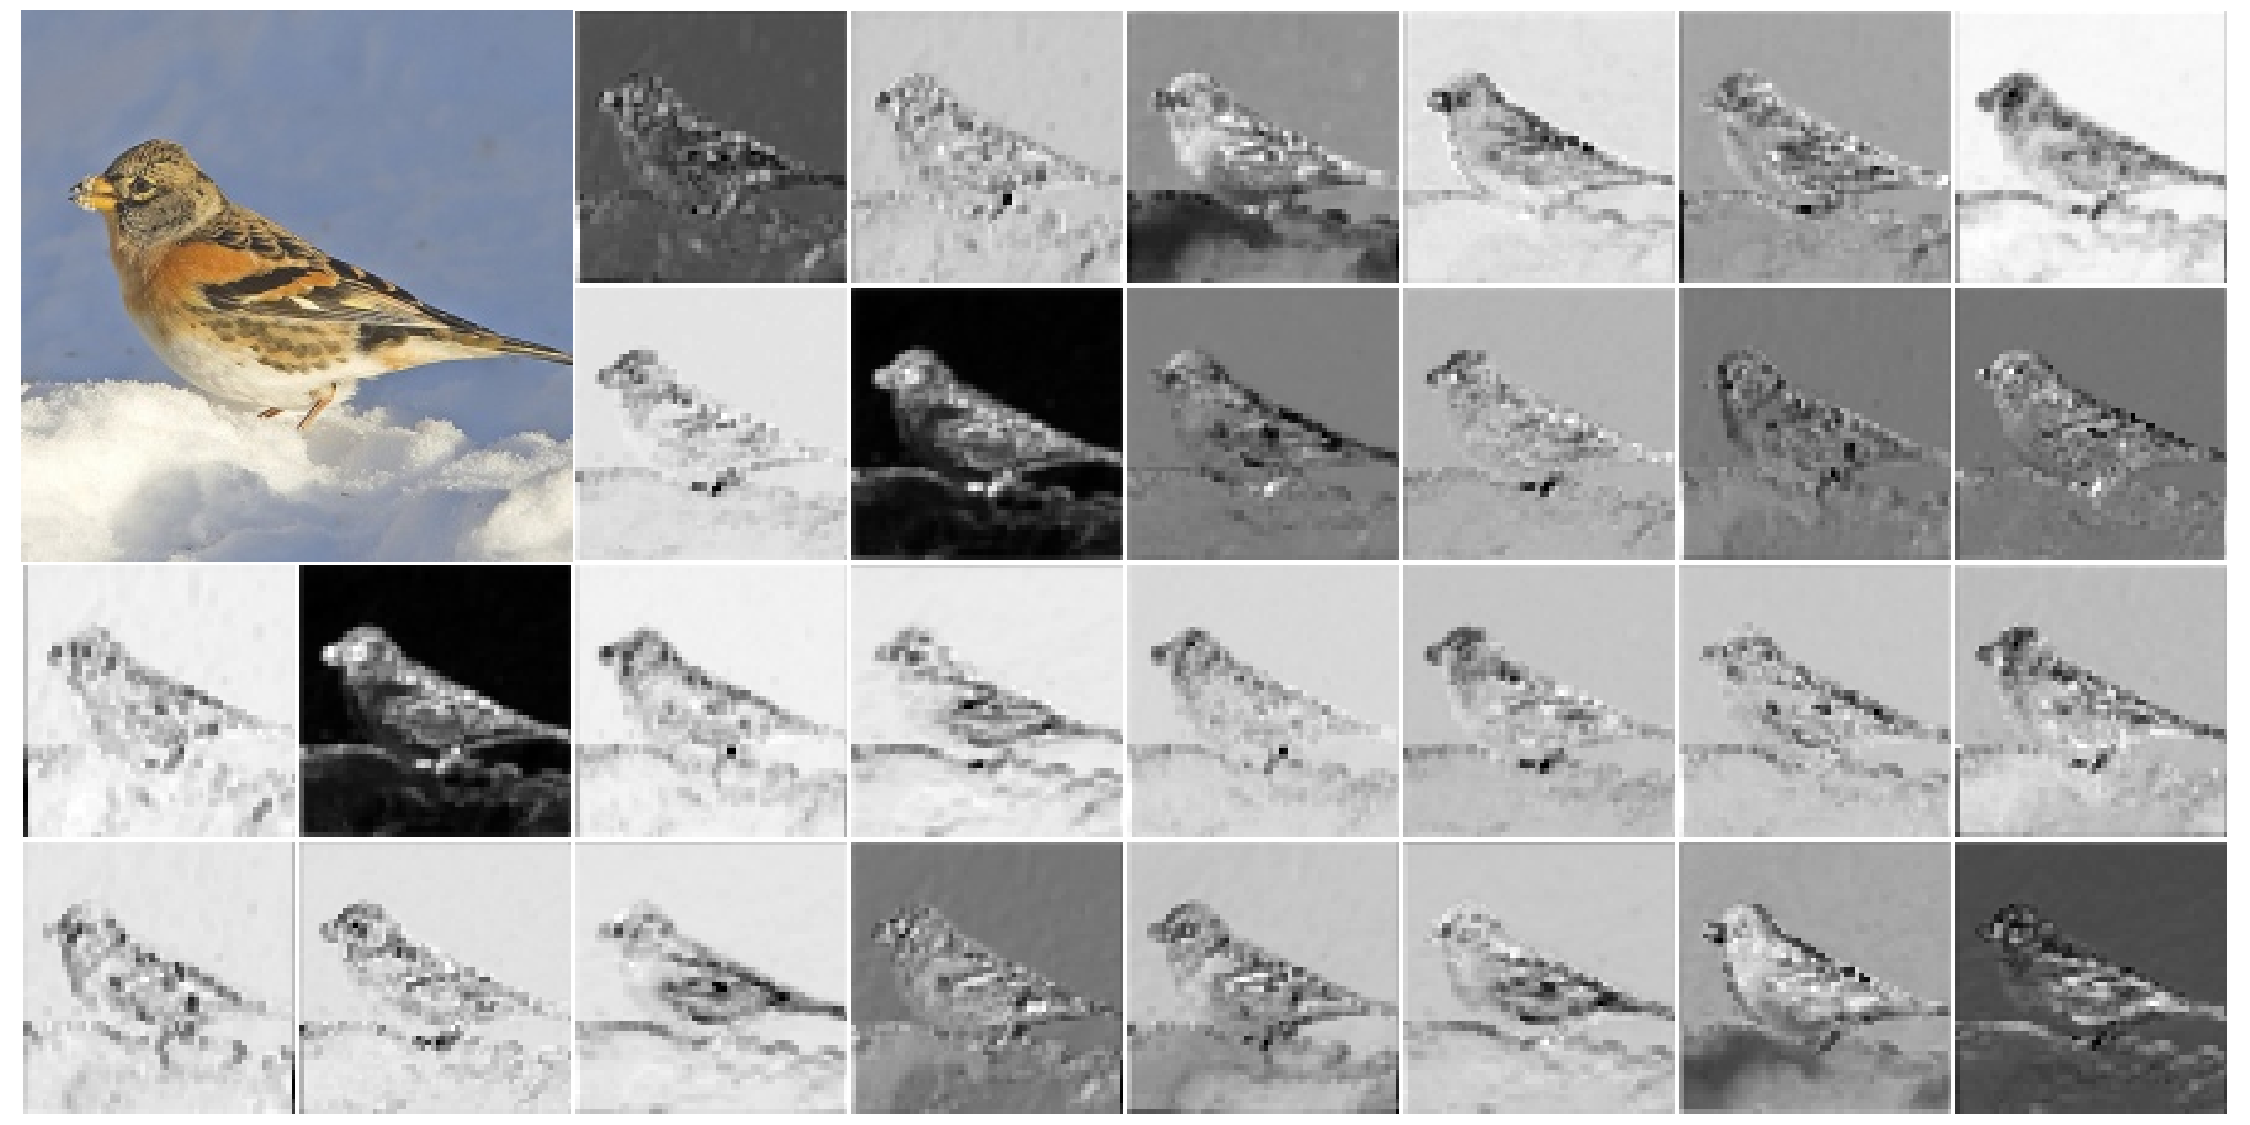
\includegraphics[width=1\linewidth]{figures/feature_layer_2.pdf}
    \vspace{-0.25in}
    \caption{Visualization of feature maps in an intermediate layer of a pre-trained ResNet50, with the top-left image as the input. Qualitatively, we can see the high redundancies across different channels. }
    \label{fig: feature_redundancy}
    \vspace{-0.05in}
\end{figure}

\subsection{Partial convolution as a basic operator}
We below demonstrate that the cost can be further optimized by leveraging the feature maps' redundancy. As visualized in~\cref{fig: feature_redundancy}, the feature maps share high similarities among different channels. This redundancy has also been covered in many other works~\cite{han2020ghostnet,zhang2020split}, but few of them make full use of it in a simple yet effective way.

\begin{figure*}
    \vspace{-0.05in}
    \centering
    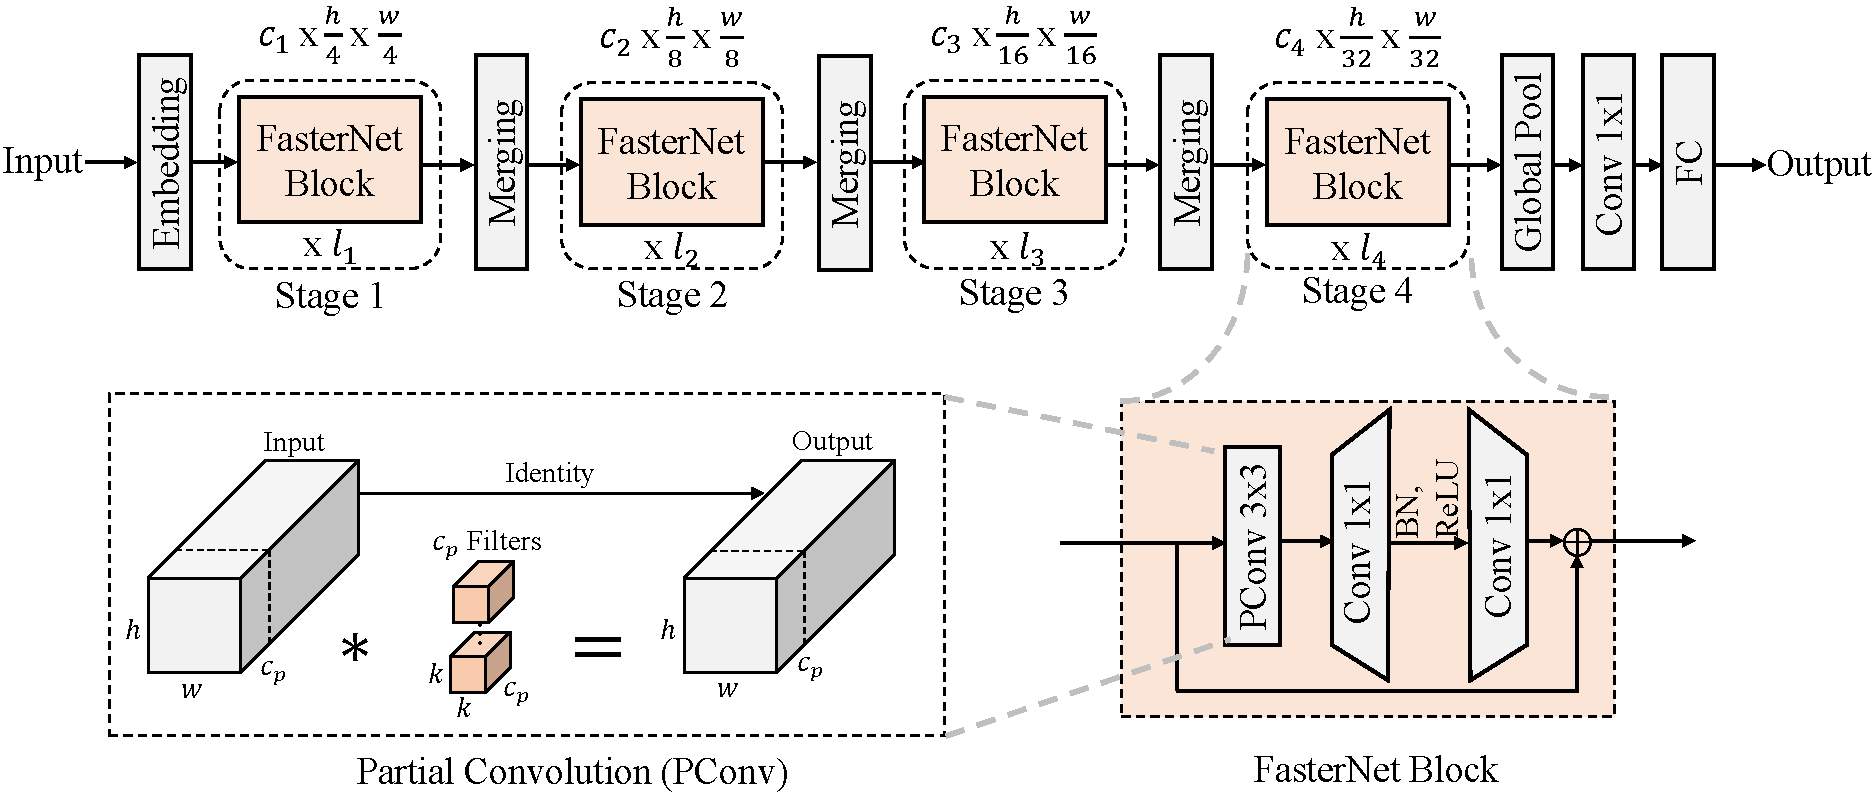
\includegraphics[width=0.83\linewidth]{figures/FasterNet-cropped.pdf}
    \vspace{-0.1in}
    \caption{Overall architecture of our FasterNet. It has four hierarchical stages, each with a stack of FasterNet blocks and preceded by an embedding or merging layer. The last three layers are used for feature classification. Within each FasterNet block, a PConv layer is followed by two PWConv layers. We put normalization and activation layers only after the middle layer to preserve the feature diversity and achieve lower latency.
    }
    \label{fig: FasterNet}
    \vspace{-0.15in}
\end{figure*}

\begin{figure}
    \centering
    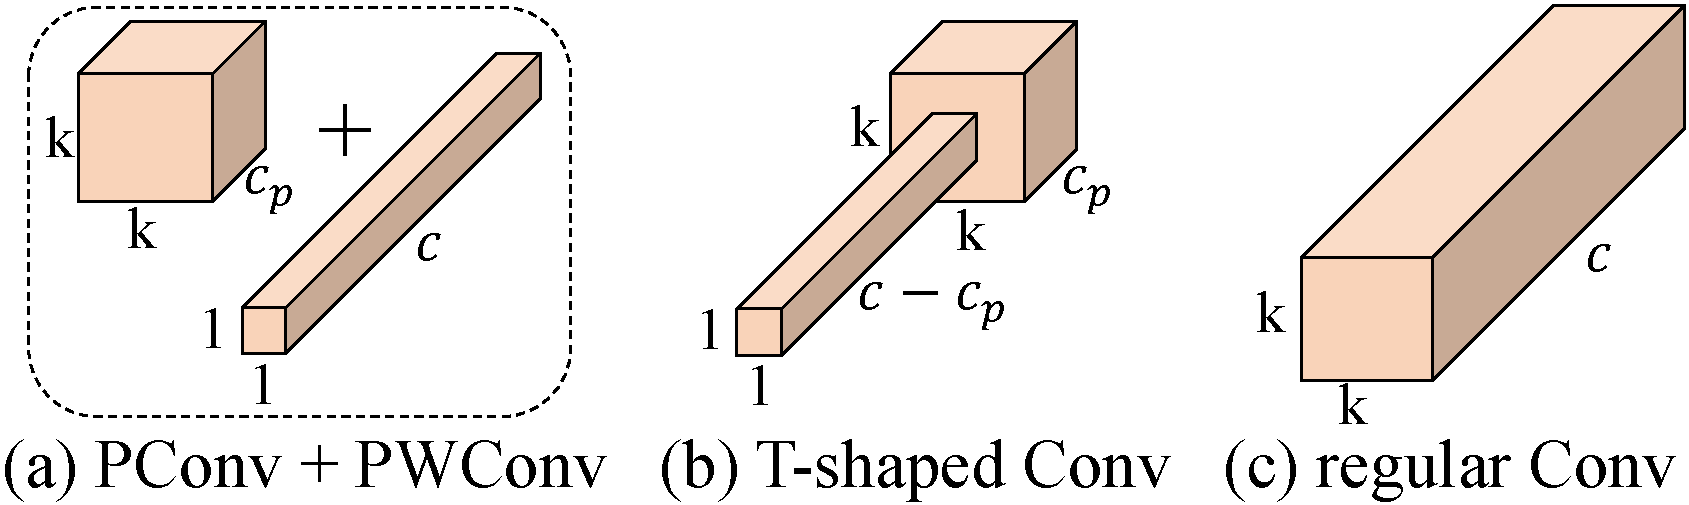
\includegraphics[width=.92\linewidth]{figures/pconv_pwconv-cropped.pdf}
    \vspace{-0.1in}
    \caption{Comparison of convolutional variants. A PConv followed by a PWConv (a) resembles a 
    T-shaped
     Conv (b), which spends more computation on the center position compared to a regular Conv (c).}
    \label{fig: pconv_pwconv}
    \vspace{-0.1in}
\end{figure}

Specifically, we propose a simple PConv to reduce computational redundancy and memory access simultaneously. The bottom-left corner in~\cref{fig: FasterNet} illustrates how our PConv works. It simply applies a regular Conv on only a part of the input channels for spatial feature extraction and leaves the remaining channels untouched. For contiguous or regular memory access, we consider the first or last consecutive $c_p$
channels as the representatives of the whole feature maps for computation. Without loss of generality, we consider the input and output feature maps to have the same number of channels. Therefore, the FLOPs of a PConv are only 
\begin{equation}
   h \times w \times k^2 \times c_p^2.
  \label{eq:FLOPs_PConv}
\end{equation}
With a typical partial ratio $r \!=\! \frac{c_p}{c} \!=\! \frac{1}{4}$,
the FLOPs of a PConv is only $\frac{1}{16}$
of a regular Conv. Besides, PConv has a smaller amount of memory access, \ie,
\begin{equation}
  h \times w \times 2c_p + k^2 \times c_p^2 \approx h \times w \times 2c_p,
  \label{eq:memory_access_PConv}
\end{equation}
which is only 
$\frac{1}{4}$
of a regular Conv for 
$r=\frac{1}{4}$. 

Since there are only $c_p$
channels utilized for spatial feature extraction, one may ask if we can simply remove the remaining $(c-c_p)$
channels? If so, PConv would degrade to a regular Conv with fewer channels, which deviates from our objective to reduce redundancy. Note that we keep the remaining channels untouched instead of removing them from the feature maps. It is because they are useful for a subsequent PWConv layer, which allows the feature information to flow through all channels.

\subsection{PConv followed by PWConv }
To fully and efficiently leverage the information from all channels, we further append a pointwise convolution (PWConv) to our PConv. Their effective receptive field together on the input feature maps looks like a 
T-shaped
Conv, which focuses more on the center position compared to a regular Conv uniformly processing a patch, as shown in~\cref{fig: pconv_pwconv}.
To justify this T-shaped
receptive field, we first evaluate the importance of each position by calculating the position-wise Frobenius norm. We assume that a position tends to be more important if it has a larger Frobenius norm than other positions. 
For a regular Conv filter
$\mathbf{F} \in \mathbb{R}^{  k^2 \times  c}$, 
the Frobenius norm at position 
$i$
is calculated by
$\left\|\mathbf{F}_{i}\right\| \!=\! \sqrt{
  \sum_{j=1}^c |f_{ij}|^2
  },
$
for $i = 1, 2, 3 ..., k^2$.
We consider a salient position to be the one with the maximum Frobenius norm.
We then collectively examine each filter in a pre-trained ResNet18, find out their salient positions, and plot a histogram of the salient positions. 
Results in~\cref{fig: positionwise_norm} show that the center position turns out to be the salient position most frequently among the filters. 
In other words, the center position weighs more than its surrounding neighbors. This is consistent with the T-shaped computation which concentrates on the center position.
 
While the
 T-shaped Conv can be directly used for efficient computation, we show that it is better to decompose the T-shaped Conv into a PConv and a PWConv because the decomposition exploits the inter-filter redundancy and  further saves FLOPs. For the same input 
 $\mathbf{I} \in \mathbb{R}^{ c \times h \times w}$ 
 and output 
 $\mathbf{O} \in \mathbb{R}^{ c \times h \times w}$,
 a T-shaped Conv's FLOPs can be calculated as 
 \begin{equation}
h \times w \times \left(k^2 \times c_p \times c + c \times \left(c - c_p\right) \right),
  \label{eq:FLOPs_tuConv}
\end{equation}
which is higher than the FLOPs of a PConv and a PWConv, \ie,
\begin{equation}
   h \times w \times ( k^2 \times c_p^2 + c^2),
  \label{eq:FLOPs_PConv_PWConv}
\end{equation}
where
$
(k^{2} - 1)c > k^{2} c_p,
$
\eg when 
$
c_p = \frac{c}{4}
$
and 
$
k = 3.
$
Besides, we can readily leverage the regular Conv for the two-step implementation.

\subsection{FasterNet as a general backbone}
Given our novel PConv and off-the-shelf PWConv as the primary building operators, we further propose FasterNet, a new family of neural networks that runs favorably fast and is highly effective for many vision tasks. We aim to keep the architecture as simple as possible, without bells and whistles, to make it hardware-friendly in general. 

We present the overall architecture in~\cref{fig: FasterNet}. It has four hierarchical stages, each of which is preceded by an embedding layer (a regular Conv $4 \times 4$ with stride 4) or a merging layer (a regular Conv $2 \times 2$ with stride 2) for spatial downsampling and channel number expanding. 
Each stage has a stack of FasterNet blocks. We observe that the blocks in the last two stages consume less memory access and tend to have higher FLOPS, as empirically validated in~\cref{FLOPS_compare}. Thus, we put more FasterNet blocks and correspondingly assign more computations to the last two stages. Each FasterNet block has a PConv layer followed by two PWConv (or Conv $1 \times 1$) layers. Together, they appear as inverted residual blocks where the middle layer has an expanded number of channels, and a shortcut connection is placed to reuse the input features. 

In addition to the above operators, the normalization and activation layers are also indispensable for high-performing neural networks.
Many prior works~\cite{he2016deep,sandler2018mobilenetv2,han2020ghostnet}, however, overuse such layers throughout the network, which may limit the feature diversity and thus hurt the performance. It can also slow down the overall computation. By contrast, we put them only after each middle PWConv to preserve the feature diversity and achieve lower latency.
Besides, we use the batch normalization (BN)~\cite{ioffe2015batch} instead of other alternative ones~\cite{ba2016layer,ulyanov2016instance,wu2018group}. The benefit of BN is that it can be merged into its adjacent Conv layers for faster inference while being as effective as the others. As for the activation layers, we empirically choose GELU~\cite{hendrycks2016gaussian} for smaller FasterNet variants and ReLU~\cite{nair2010rectified} for bigger FasterNet variants, considering both running time and effectiveness. The last three layers, \ie a global average pooling, a Conv $1 \times 1$, and a fully-connected layer, are used together for feature transformation and classification.

To serve a wide range of applications under different computational budgets, we provide tiny, small, medium, and large variants of FasterNet, referred to as FasterNet-T0/1/2, FasterNet-S, FasterNet-M, and FasterNet-L, respectively. They share a similar architecture but vary in depth and width. Detailed architecture specifications are provided in the appendix.

\begin{figure}
    \vspace{-0.15in}
    \centering
    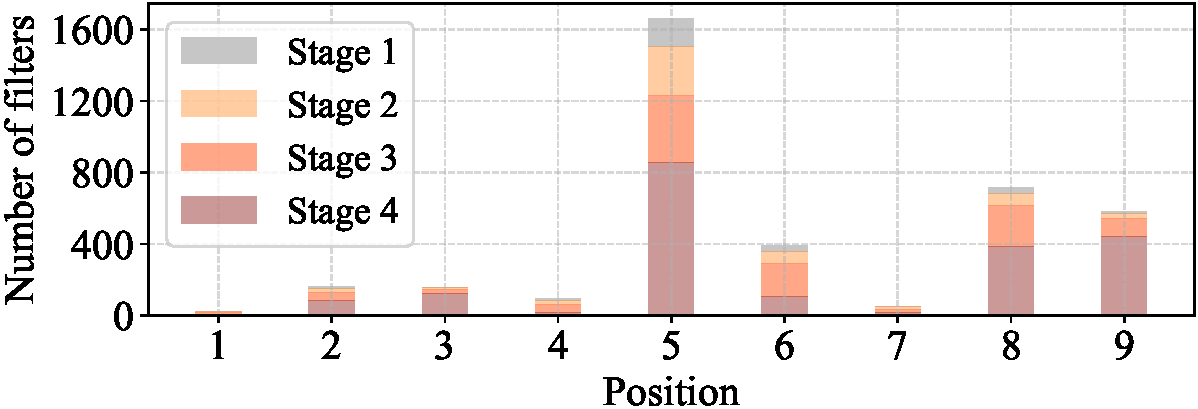
\includegraphics[width=.99\linewidth]{figures/positionwise_norm_filter-cropped.pdf}
    \vspace{-0.1in}
    \caption{Histogram of salient position distribution for the regular Conv 
    $3 \times 3$
    filters in a pre-trained ResNet18. The histogram contains four kinds of bars, corresponding to different stages in the network. In all stages, the center position (position 5) appears as a salient position most frequently.}
    \label{fig: positionwise_norm}
    \vspace{-0.1in}
\end{figure}
